\documentclass[11pt]{article} %{{{

\usepackage{amsmath}
\usepackage{amssymb}
\usepackage{graphicx}
\usepackage{url}
\usepackage[usenames,dvipsnames,svgnames,table]{xcolor}
\definecolor{light-gray}{gray}{0.8}
\def \del #1{ {\color{light-gray}{#1}} }
\def\yy#1{\footnote{\color{red}\textbf{#1 -YY}} }
\usepackage{hyperref}


\usepackage[backend=bibtex]{biblatex}
\addbibresource{main.bib}
\graphicspath{ {./figs} }

\usepackage{array}

%}}}

\begin{document} %{{{

\title{Evolution of Fanfictions in Fandoms} %{{{
\date{\today}
\maketitle %}}}

\section{Introduction} %{{{
\label{sec:introduction}
\paragraph{} Many communities in the Internet are formed by a group of people sharing common interests. In particular, the contemporary pop culture sees the rise of a specific kind of online communities - fandoms. Fandoms, by convention, are a group of people that identify, connect and interact with each other based on a similar interest, such as a movie, a book or a band \cite{wiki:fandom}. 

\paragraph{}Transformative works, or in a more common term, fan works, are one typical kind of production from fandoms\cite{wiki:transf_work}. These are creative works made by fans based on one or more original works, and are often centered around certain characters or story lines. For example, a story written by a contemporary fan about Sherlock Holmes in his retirement is considered a fan fiction in the Sherlock Holmes fandom. Although fan works contain multiple media types such as art, music and games, one of the most common type is creative writing--fanfictions.

\paragraph{} This project studies the evolution of fanfictions in fandoms. Data for the study comes from Archive of Our Own (AO3). This site hosts fan works --- mainly fanfictions --- that users upload and their metadata, and categorizes them based on fandoms. Established in 2010, it has become one of the most popular transformative work archives. We collected fanfictions from 42 fandoms according to AO3's list of most popular fandoms as of March 2016 \footnote{from this list: \url{http://archiveofourown.org/media}}. We only kept the fictions written in English, which leaves us with 3,726,307 fictions. The number of fictions in each fandom is shown in Figure \ref{fig: fandom_size}.


\begin{figure}[htbp]
\begin{center}
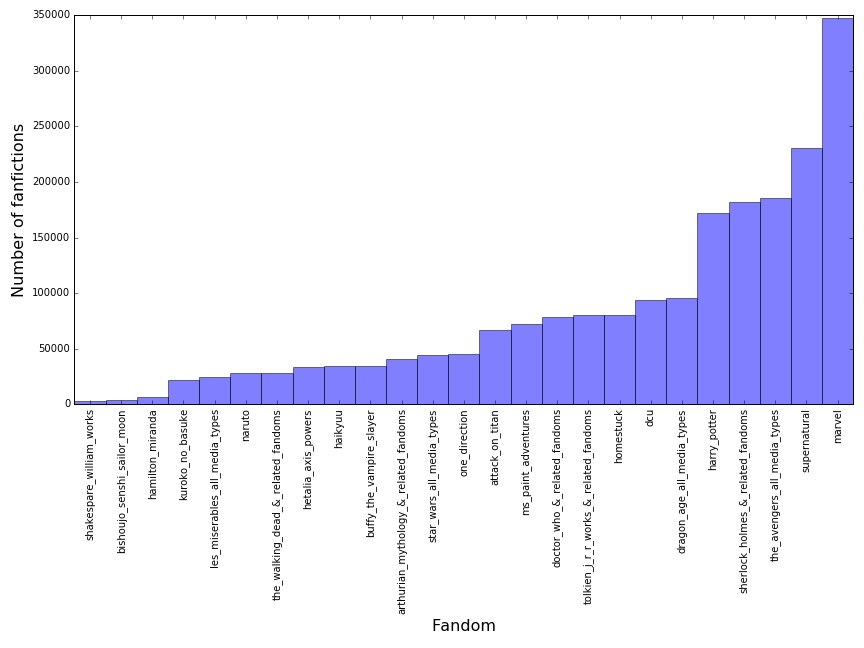
\includegraphics[width=0.8\textwidth]{/fandom_size.png}
\caption{Number of fanfictions in each fandom}
\label{fig:fandom_size}
\end{center}
\end{figure}


\paragraph{} Besides the work texts, we also collected metadata including 23 fields that can be roughly divided into two categories. One is tags generated by the author, which describes the works' contents; the other is tags that are automatically generated, and describes the works’ other information, as well as the readers' feedback. Table \ref{tab:metadata} gives the names of these fields. 

\begin{table}[htp]
\caption{Metadata of the writings}
\begin{center}
\begin{tabular}{p{3cm}|p{3cm}|p{3cm}|p{3cm}}
  \hline			
 \multicolumn{2}{c}{ Content related} & \multicolumn{2}{c}{Non-content related}\\ 
 User-generated & Not-user-generated &  User-generated & Not-user-generated \\
\hline
Additional Tags, Characters, Relationship, Summary, Text, Title
 & Fandoms,  Archive Warnings, Category, Rating
& Author, Notes
& Bookmarks, Chapter Index, Chapters, Comments, Complete Date, Hits, Kudos, Language, Publish Date, Update Date, Word Count\\
\hline
\end{tabular}
\end{center}
\label{tab:metadata}
\end{table}%

\paragraph{} Among the metadata fields, we're especially interested in the Kudos field, which shows how many times a fiction has been ``liked" by readers. This is a useful proxy for the popularity of a piece of work in a specific fandom.

\paragraph{} We model the fictions with a unigram language model. The Good-Turing smoothing\cite{gales1995good} is applied to assign non-zero probabilities to previously unseen unigrams. When creating the unigram list, we also remove the rare unigrams that only appear once.

\paragraph{} This transformation allows us to apply many text analysis methods. We choose to use the Kullback--Leibler divergence to measure the distance between texts. Under this measurement, fictions from the same author are more similar and have a smaller KL divergence between each other, compared to fictions from different authors, as shown in Figure \ref{fig:kl_comp}.


\begin{figure}[htbp]
\begin{center}
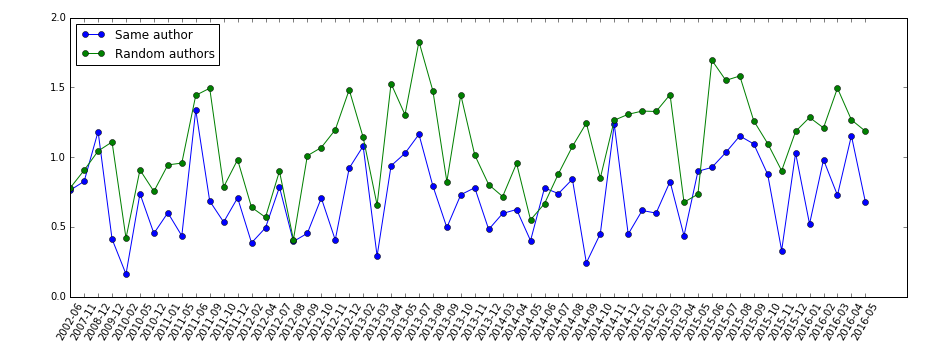
\includegraphics[width=\textwidth]{/kl_comparison.png}
\caption{KL divergence between fictions from the same author and fictions from different authors in the Shakespeare fandom. In each time slice, an author with 5 or more fictions is selected. The average KL divergence between each pair of his/her fictions is them computed. The computation is then repeated on a random example with the same size. }
\label{fig:kl_comp}
\end{center}
\end{figure}

\paragraph{} We further define the concept of a \emph{standard work}. A standard work of a time period is the average of probability distributions of all works in that time period. This allows us to calculate the KL divergence between a work and the standard work. We then attempt to analyze the relation between a fiction's distance to the stand work and the kudos that it receive. Figure \ref{fig:kl_kudos} shows that the kudos peak with the KL divergence slightly below a z-score of 0, that is, when the fiction is a little more similar to the standard work than average. However, besides this there seems not to be a consistent pattern across fandoms.

\begin{figure}[htbp]
\begin{center}
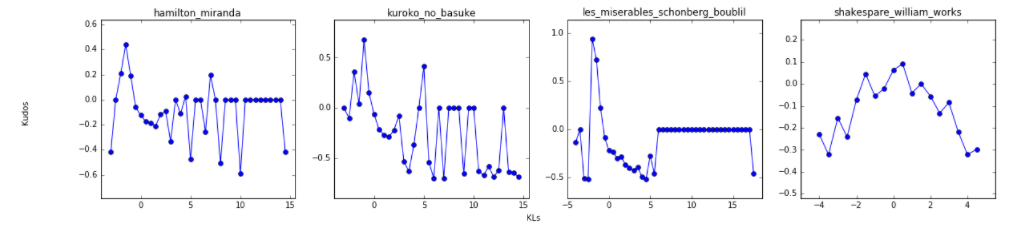
\includegraphics[width=\textwidth]{/kl_kudos_4fandoms.png}
\caption{Relation between fictions' KL divergence to standard work and their kudos in 4 fandoms. Both statistics are turned into z-scores. Highest kudos show up with z-score of the KL divergence slightly below zero.}
\label{fig:kl_kudos}
\end{center}
\end{figure}

%}}}





\section{Results} %{{{
\label{sec:results}

%}}}

\section{Methods} %{{{
\label{sec:methods}

%}}}

\printbibliography
    
\end{document} %}}}
